%%%%%%%%%%%%%%%%%%%%%%%%%%%%%%%%%%%%%%%%%%%%%%%
%%%%%%%%%%%%%%%%%%%%%%%%%%%%%%%%%%%%%%%%%%%%%%%
\section{Background}
\subsection{CUDA}

\begin{frame}
    \begin{block}{Compute Unified Device Architecture}
        \begin{itemize}
            \item CUDA is a parallel programming model developed by NVIDIA, which allows developers 
            to leverage the power of GPUs for general-purpose computing.
            \item CUDA programs are written in C/C++ and executed on the GPU.
        \end{itemize}
        \begin{center}
            \begin{figure}[H]
                
\includegraphics[scale=0.5]{figures/Cuda.png}
            \end{figure}
        \end{center}        
    \end{block}
\end{frame}

\begin{frame}{Graphics Processing Units (GPUs)}
	\begin{block}{}
		\begin{itemize}
			\item GPUs are designed for massive parallelism, while CPUs focus on sequential processing.
            \item GPUs are designed to handle massive amounts of data and perform the same operation on them simultaneously.
		\end{itemize}
        \begin{center}
            \begin{figure}[H]
                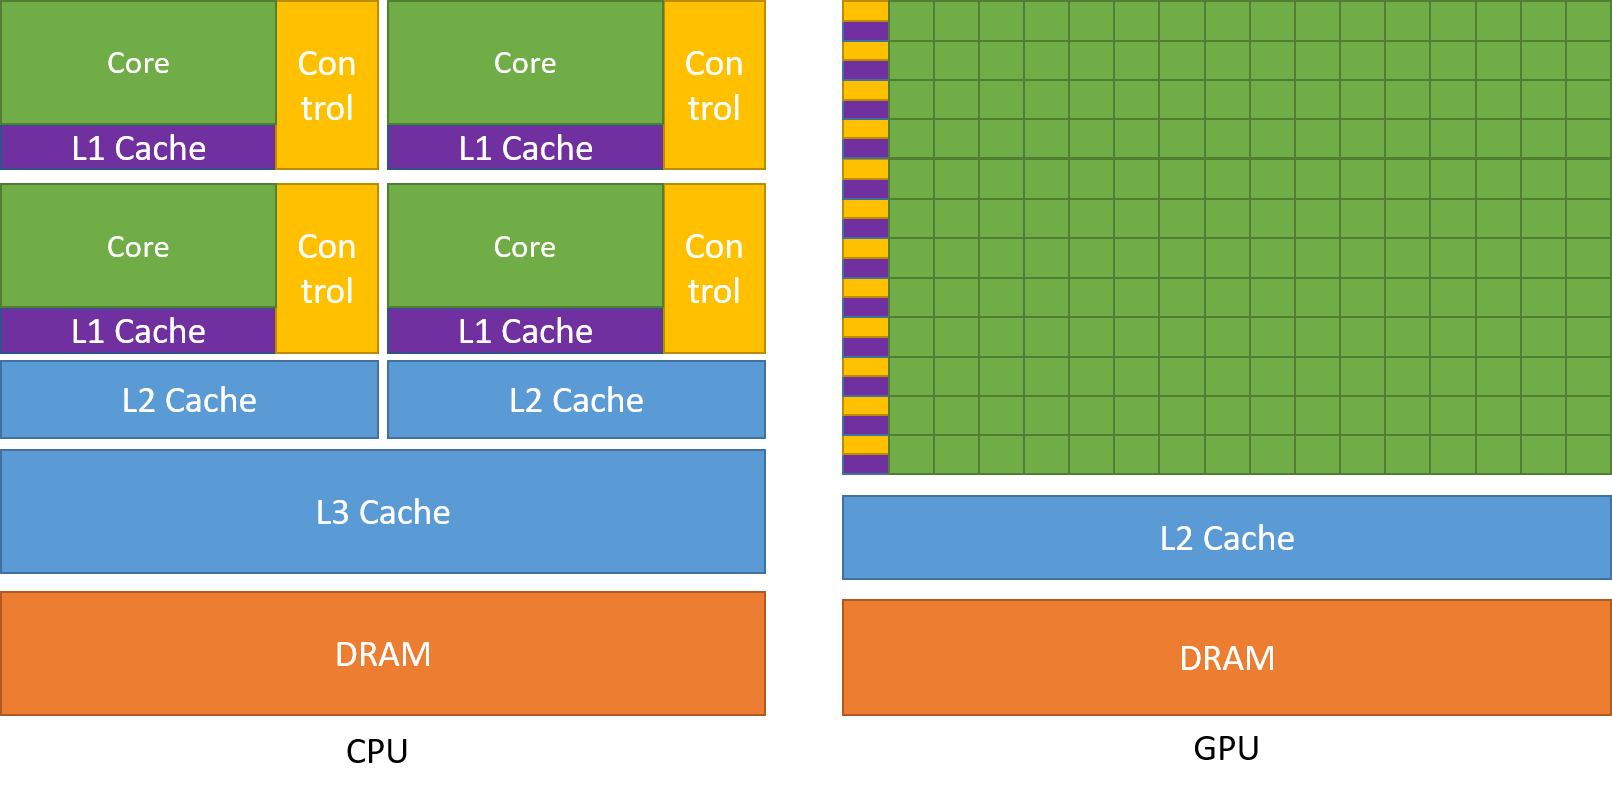
\includegraphics[scale=0.3]{figures/gpu-devotes-more-transistors-to-data-processing.png}
            \end{figure}
        \end{center}
	\end{block}
\end{frame}

\begin{frame}{GPU Microarchitecture}
    \begin{block}{}
        \begin{itemize}
            \item Streaming Multiprocessor (SM): An SM is a processing unit in a GPU that executes multiple threads concurrently. 
            It contains ALUs, registers, and shared memory, and is essential for parallel computations.
            \item Warp: A warp is a group of threads (typically 32) in a GPU that are executed simultaneously using SIMD. 
            All threads in a warp perform the same instruction on different data elements, maximizing throughput.
            \item SIMD (Single Instruction, Multiple Data): SIMD is a computing paradigm where one instruction is applied to multiple data elements concurrently. 
            GPUs use SIMD in warps for efficient parallel execution.
        \end{itemize}
        \begin{center}
            \begin{figure}[H]
                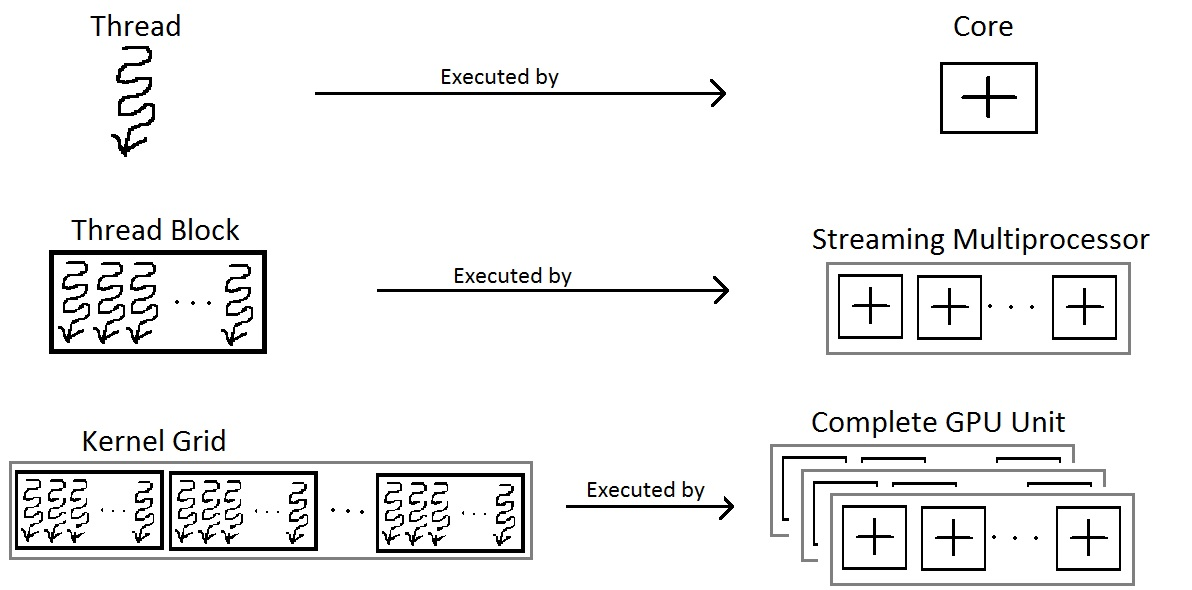
\includegraphics[scale=0.35]{figures/Software-Perspective_for_thread_block.jpg}
            \end{figure}
        \end{center}
    \end{block}
\end{frame}

\begin{frame}{CUDA Programming Model}
    \begin{block}{}
        \begin{itemize}
            \item Kernels
            \item Threads
            \item Kernel Launch Parameters
        \end{itemize}
        \begin{center}
            \begin{figure}[H]
                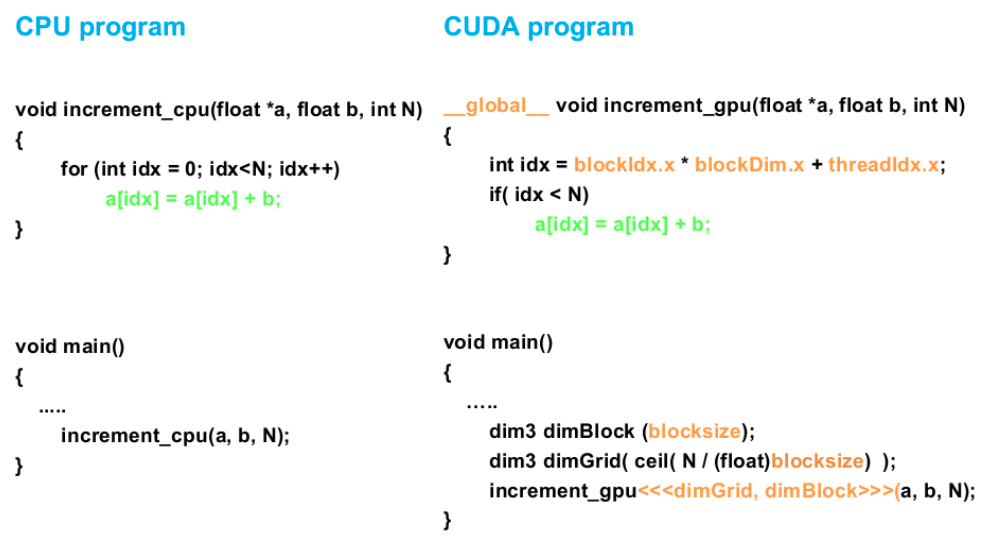
\includegraphics[scale=0.3]{figures/CPUvsGPUprogram.png}
            \end{figure}
        \end{center}
    \end{block}
\end{frame}

\begin{frame}[fragile]{Kernels}
	\begin{block}{}
        \begin{minted}{c}
// Kernel definition
__global__ void VecAdd(float* A, float* B, float* C)
{
    int i = threadIdx.x;
    C[i] = A[i] + B[i];
}

int main()
{
    ...
    // Kernel invocation with N threads
    VecAdd<<<1, N>>>(A, B, C);
    ...
}
        \end{minted}
    \end{block}            
\end{frame}

\begin{frame}{Thread Hiearchy}
	\begin{block}{}
        \begin{itemize}
            \item Threads constitute the basic units of parallel execution and 
            are organized within a hierarchical structure encompassing threads, thread blocks, and grids.
            \item Blocks can be executed in any order, both concurrently and sequentially, across the available 
            SMs on a GPU.
        \end{itemize}
        \begin{center}
            \begin{figure}[H]
                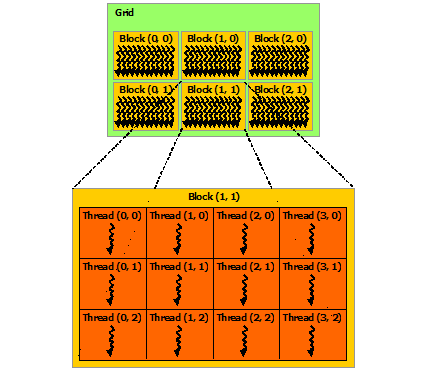
\includegraphics[scale=0.65]{figures/grid-of-thread-blocks.png}
            \end{figure}
        \end{center}
    \end{block}
\end{frame}

\begin{frame}[fragile]{Kernel Launch Parameters}
	\begin{block}{}
        \begin{itemize}
            \item Kernel launch parameters define the organization of threads and blocks for a particular kernel invocation.
            \item Optimal kernel launch parameters can significantly improve the performance of a GPU program.
            \item Finding the best kernel launch parameters is not straightforward, as they depend on the data, 
            hardware, and program characteristics.
        \end{itemize}
        \begin{minted}{c}
    //a CUDA kernel for vector addition
    __global__ void vector_addition(int *A, int *B, size_t n) {
        A[threadIdx.x] += B[threadIdx.x];
    }
    int main(){
        ...
        //launch the kernel with 1 block and n threads per block
        vector_addition<<<1, n>>>(Ad, Bd, n);
        ...
    }			
        \end{minted}
	\end{block}
\end{frame}

\begin{frame}{Heterogeneous Programming Mode}
    \begin{center}
        \begin{figure}[H]
            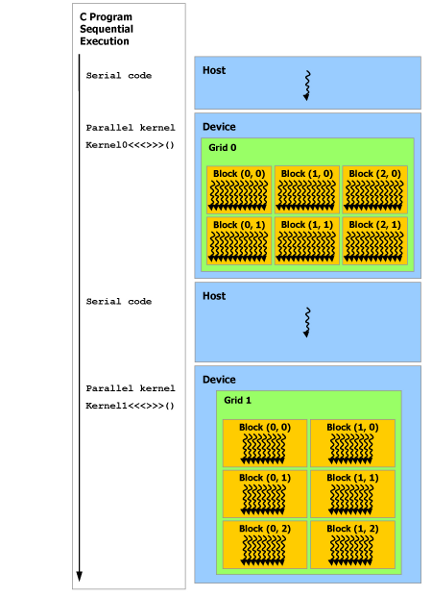
\includegraphics[scale=0.5]{figures/heterogeneous-programming.png}
        \end{figure}
    \end{center}
\end{frame}

\begin{frame}{CUDA Memory Model}
    \begin{center}
        \begin{figure}[H]
            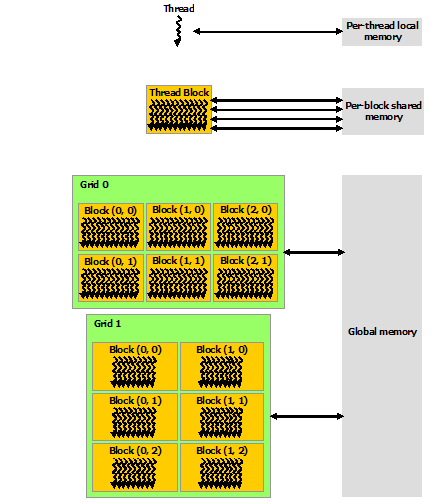
\includegraphics[scale=0.55]{figures/memory-hierarchy.png}
        \end{figure}
    \end{center}
\end{frame}

\subsection{MWP-CWP}
\begin{frame}[fragile]{Main observation of MWP-CWP}
	\begin{block}{}
        As we know, memory accesses can be overlapped between warps.
        \begin{center}
            \begin{figure}[H]
                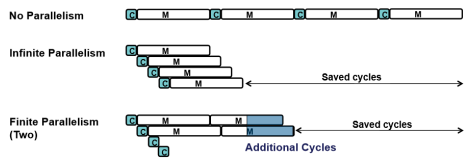
\includegraphics[scale=0.6]{figures/mwp_cwp.png}
            \end{figure}
        \end{center}
        Performance can be predicted by knowing the amount of memory-level parallelism.
    \end{block}
\end{frame}

\begin{frame}[fragile]{Memory Warp Parallelism (MWP)}
	\begin{block}{}
        MWP is the maximum number of warps that can overlap memory accesses.
        \begin{center}
            \begin{figure}[H]
                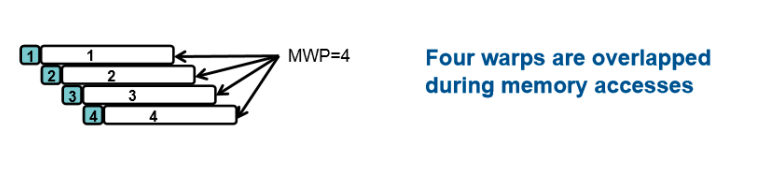
\includegraphics[scale=0.4]{figures/MWP.png}
            \end{figure}
        \end{center}
        \begin{itemize}
            \item MWP = 4.
            \item MWP is determined by \#Active SMs, \#Active warps, Bandwidth, Types of memory accesses (Coalesced, Uncoalesced)
        \end{itemize}
    \end{block}
\end{frame}

\begin{frame}[fragile]{Computation Warp Parallelism (CWP)}
	\begin{block}{}
        CWP is the number of warps that execute instructions during one memory access period plus one.
        \begin{center}
            \begin{figure}[H]
                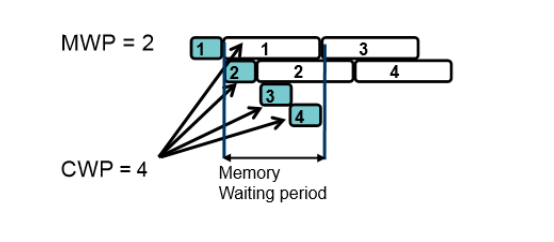
\includegraphics[scale=0.5]{figures/CWP.png}
            \end{figure}
        \end{center}
        \begin{itemize}
            \item CWP = 4.
        \end{itemize}
    \end{block}
\end{frame}

\begin{frame}{$MWP \leq CWP$}
	\begin{block}{}
        \begin{center}
            \begin{figure}[H]
                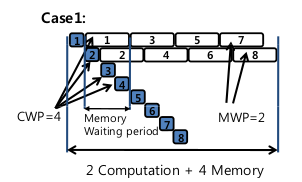
\includegraphics[scale=0.65]{figures/cwpgreater.png}
            \end{figure}
        \end{center}
        \begin{itemize}
            \item Computation cycles are hidden by memory waiting periods
            \item Overall performance is dominated by the memory cycles
        \end{itemize}
    \end{block}
\end{frame}

\begin{frame}{$MWP > CWP$}
	\begin{block}{}
        \begin{center}
            \begin{figure}[H]
                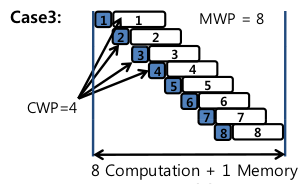
\includegraphics[scale=0.65]{figures/mwpgreater.png}
            \end{figure}
        \end{center}
        \begin{itemize}
            \item Memory accesses are mostly hidden due to high MWP
            \item Overall performance is dominated by the computation cycles
        \end{itemize}
    \end{block}
\end{frame}

\begin{frame}{Questions to answer}
	\begin{block}{}
		\begin{itemize}
			\item For a CUDA program, can we automatically and dynamically finds the values of kernel launch parameters which optimize the performance for each kernel invocation independently?
		\end{itemize}
	\end{block}
\end{frame}


%%%%%%%%%%%%%%%%%%%%%%%%%%%%%%%%%%%%%%%%%%%%%%%
%%%%%%%%%%%%%%%%%%%%%%%%%%%%%%%%%%%%%%%%%%%%%%%
